\documentclass[11pt,fontset=fandol,a4paper]{ctexart}

\usepackage[a4paper,left=2.5cm,right=2.5cm,top=2.8cm,bottom=2.8cm]{geometry}
\usepackage{amsmath,amssymb}
\usepackage{booktabs,threeparttable,array,multirow}
\usepackage{graphicx}
\usepackage{caption}
\usepackage{float}
\usepackage{fancyhdr}
\usepackage{setspace}
\usepackage{xcolor}
\usepackage{hyperref}
\usepackage{enumitem}
\usepackage{tabularx}

\hypersetup{colorlinks=true,linkcolor=blue!60!black,citecolor=blue!60!black,urlcolor=blue!60!black}
\graphicspath{{../output/paper_plan_core/figures/}{output/paper_plan_core/figures/}}
\onehalfspacing
\pagestyle{fancy}
\fancyhf{}
\fancyfoot[R]{\thepage}
\renewcommand{\headrulewidth}{0pt}
\renewcommand{\footrulewidth}{0pt}
\fancypagestyle{plain}{
  \fancyhf{}
  \fancyfoot[R]{\thepage}
  \renewcommand{\headrulewidth}{0pt}
  \renewcommand{\footrulewidth}{0pt}
}

% 金融研究风格的节标题格式
\ctexset{
  section/format = \centering\bfseries\zihao{4},
  section/name = {,、},
  section/number = \chinese{section},
  subsection/format = \bfseries\zihao{-4},
  subsection/name = {（,）},
  subsection/number = \chinese{subsection},
}

\title{谁受益，谁受损？\\大语言模型发布的AI生态位置再定价效应}
\author{陈茁 \quad 鲁睿爽\thanks{陈茁，山东大学经济研究院，zhuochen@sdu.edu.cn。鲁睿爽，山东大学经济研究院。}}
\date{}

\begin{document}
\renewcommand{\thefootnote}{\fnsymbol{footnote}}
\maketitle
\setcounter{footnote}{0}
\renewcommand{\thefootnote}{\arabic{footnote}}

\begin{abstract}
\noindent 大语言模型（LLM）的密集发布正在重塑人工智能产业链的利润分配格局，但现有研究缺乏对其资本市场外溢效应的系统性实证考察。本文以2024--2026年60次重大AI模型发布事件为外生冲击，以双盲编码建立的8维AI生态位置编码体系（Cohen's $\kappa=0.986$）刻画企业的产业链角色，基于86家美股上市公司构建5\,160条事件--公司层面观测，采用事件研究法考察模型发布沿产业链生态位置产生的异质性市场反应。研究发现：（1）模型发布沿生态位置产生方向相反的价值再分配，上游硬件公司在$CAR[0,+20]$窗口获得$+2.28$个百分点的累计异常收益（$p<0.01$），部署型下游公司则损失$-1.90$个百分点（$p<0.01$），上下游"剪刀差"约4.7个百分点；（2）上游硬件溢价仅在闭源模型发布时成立（$+3.07\%$），开源模型发布时该溢价消失甚至逆转（$-0.59\%$），交互项显著（$p=0.018$）；（3）控制模型能力指标后位置效应不变甚至增大，表明生态位置是一个独立于技术特征的市场定价维度。

\vspace{0.5em}
\noindent 关键词：大语言模型；事件研究；产业链外溢；生态位置；开源与闭源

\vspace{0.3em}
\noindent JEL分类号：G14\quad O33\quad L14
\end{abstract}

%% ========================================
\section{引言}
%% ========================================

2025年1月20日，中国人工智能初创企业深度求索（DeepSeek）在GitHub上发布了开源推理模型DeepSeek R1及其技术报告，既无新闻发布会，亦无媒体预热，模型权重直接公开上传。该模型据称训练成本约600万美元，低于OpenAI同期旗舰模型估计训练成本的百分之一，而其推理性能在多项主流基准测试上与OpenAI的o1相当，有时甚至超越。消息在技术社区迅速传播，并触发市场对大规模专有算力需求预期的重新评估。2025年1月27日，NVIDIA股价单日下跌16.9\%，市值蒸发约5\,900亿美元，\footnote{数据来源：Bloomberg。NVIDIA于2025年1月27日（美东时间）收盘价较前一交易日下跌16.86\%，对应市值从约3.49万亿美元降至约2.90万亿美元。}创下美股历史上单只股票单日市值损失纪录；同日Broadcom跌8.1\%，ARM跌10.2\%，Marvell跌10.7\%，上游半导体板块整体承压。与此同时，以云端服务和应用部署为主业的部分企业跌幅明显小于半导体板块，部分依赖低成本开源模型降低采购支出的企业甚至当日收涨。这一单日市场截面呈现出一个值得系统研究的现象：同属AI产业链的企业，在面对同一技术事件时，展现出方向相反的市场反应，上下游估值走势取决于企业在产业链中所处的生态位置。

那么，这种分化是偶然的，还是模型发布反复触发的系统性现象？围绕AI如何影响经济，现有讨论中存在几组相互对立的判断。第一组判断涉及AI与现有生产活动的关系：一种观点认为AI提升企业和劳动者的生产效率，使用AI的企业由此获得竞争优势，技术进步因而具有普遍的正外部性；另一种观点认为AI替代而非辅助现有的产品、服务和岗位，技术进步因而会压缩可被模型直接替代的企业的生存空间。第二组判断涉及技术能力的分布：一种观点认为AI正在降低生产能力的门槛，个人凭借AI工具即可完成此前需要团队协作才能完成的工作；另一种观点认为算力仍是决定性的制约因素，少数掌握先进芯片和云端基础设施的厂商因此占据了技术进步带来的大部分收益。第三组判断涉及技术变革的整体后果：一种观点认为技术边界的拓展具有普遍的正向效应，能力提升会沿产业链扩散，使更广泛的参与者从中受益；另一种观点认为每一次技术变革都伴随利益分配格局的调整，谁能从中获益、谁的地位被削弱，取决于参与者在新格局中所处的位置。这三组判断各自隐含不同的赢家和输家，但较少在同一事件中被对照检验。同一次技术冲击下，不同公司的市场反应为何会出现方向相反的情形，又是什么决定了谁受益、谁受损？本文的核心问题由此分为两层，其一是大语言模型发布究竟是AI产业链的普遍利好，还是沿生态位置产生方向相反的价值再定价；其二是若存在位置异质性，这种再分配的方向、幅度与边界条件是什么。

相关文献已在三条脉络上提供了初步基础。技术事件可通过资本市场重新定价企业预期现金流（MacKinlay, 1997；Chen et al., 2005）；AI进展可被股权市场定价，且高暴露企业与低暴露企业的反应存在差异（Eisfeldt et al., 2023；Blomkvist et al., 2023）；产业链成员公告可沿供应链传导并产生异质反应（Cohen \& Frazzini, 2008；Gofman et al., 2020）。\footnote{详细的文献综述见第二节。}然而，现有研究缺乏对同一AI冲击如何沿生态位置产生方向相反效应的系统考察，开源与闭源属性如何调节传导方向也尚无股权市场层面的直接证据。与本文最接近的研究是Bjorkegren（2025），其发现开放权重与闭源AI发布对美国长期债券利率的影响方向相反；本文在股权市场横截面提供互补证据，并将研究从单次事件扩展至60次系统性样本。

有鉴于此，本文以2024年4月至2026年3月间60次重大AI模型发布事件为准自然实验，结合86家美股上市AI相关企业，构建5\,160条事件--公司层面观测，采用事件研究法系统考察模型发布沿生态位置产生的异质性市场反应。为精准刻画企业在AI产业链中的角色，本文构建了一套8维生态位置编码体系，涵盖上游硬件、上游云服务、下游集成、下游部署、下游赋能、直接竞争者等维度，并通过双盲编码与仲裁流程形成高信度最终数据（汇总Cohen's $\kappa=0.986$），为本文及后续研究提供可追溯、可复用的产业链测量工具。

本文的实证结果表明，上述判断均只反映了部分事实，模型发布同时具有技术互补效应和技术替代效应，分别作用于产业链的不同位置，权力流向的方向也取决于模型的开闭源属性，而非单一方向决定。第一，模型发布沿生态位置产生方向相反的价值再分配。模型能力的提升对上游而言意味着更确定的算力需求，二者构成互补关系；对下游而言，更强的模型意味着自身的部分业务功能可被模型直接替代，二者构成替代关系，上游和下游对同一次技术冲击的反应方向因此相反。上游硬件企业在$CAR[0,+20]$窗口获得$+2.28$个百分点的显著正向异常收益（$p<0.01$），部署型下游企业则损失$-1.90$个百分点（$p<0.01$），上下游差异约4.7个百分点；以2024年末样本企业平均市值折算，这一差异在单次事件后的20个交易日内对应数十亿至上百亿美元的估值差额。第二，上游硬件溢价的存在依赖于模型的开闭源属性。闭源模型只能通过发布方的API获取，其训练和推理依赖发布方自有或采购的专有算力，直接巩固上游硬件供应商的需求确定性；开源模型权重公开，任何主体均可部署，且通常伴随更高的推理效率，使同等能力所需的算力下降，上游硬件供应商的边际价值因此被削弱。闭源模型发布时上游硬件企业获得$+3.07\%$的超额收益，开源模型发布时该溢价消失甚至逆转为$-0.59\%$（不显著），交互项在统计上显著（$p=0.018$），Wild Bootstrap检验支持这一结果的稳健性。第三，控制模型能力评分后，上述位置效应不仅未减弱，反而有所扩大。能力更强的模型本身会引发一部分全行业普遍受益的预期，这部分预期的方向与位置效应相反，在基准回归中部分抵消了位置效应的幅度；剥离能力变异后，生态位置作为独立定价维度的信号更加清晰，说明市场对AI生态的重新定价并非完全由技术进步本身驱动，企业在产业链中所处的位置本身构成一个独立的定价依据。

相较于已有研究，本文的边际贡献主要体现在以下三个方面。其一，本文将AI技术冲击的资本市场研究从"平均暴露度"推进到"产业链位置异质性"。以Eisfeldt et al.（2023）为代表的研究以暴露度高低对企业排序，能够识别AI浪潮的总体受益方，但无法区分同样"暴露度高"的硬件供应商与应用部署商在同一冲击下的截然不同命运；本文的生态位置编码框架打开了这个黑箱，首次在系统性样本中提供方向相反、数量可比的异质反应证据。其二，本文将开源/闭源属性从技术治理变量提升为产业链利润分配变量，揭示了开源大模型通过削减独占式算力需求预期从而逆转上游溢价这一机制；这一发现直接联系了Bommasani et al.（2021）关于基础模型治理与下游传导的讨论，并在股权市场层面补充了Bjorkegren（2025）的债券市场证据。其三，在方法论层面，本文构建了可审计、多维、高信度的AI生态位置编码体系（Cohen's $\kappa=0.986$），与Kogan et al.（2017）利用专利文本测量创新私人价值的精神一脉相承，为后续研究测量企业AI产业链角色提供了可复用基础设施。

本文其余部分安排如下：第二部分梳理相关文献并推导研究假说；第三部分介绍研究设计；第四部分报告基准实证结果；第五部分进行稳健性检验；第六部分展开进一步分析与机制讨论；第七部分总结全文。


%% ========================================
\section{文献综述与研究假说}
%% ========================================

\subsection{科技产品发布与技术创新事件研究}

技术事件如何进入资产价格，是金融学使用事件研究法回答的经典问题。Fama et al.（1969）最早用股票分拆检验价格对新信息的调整，Brown \& Warner（1985）系统讨论了日收益率事件研究的检验性质，MacKinlay（1997）和Kothari \& Warner（2007）进一步把事件研究法整理为估计公告信息含量的标准工具。这一传统的共同前提是，在交易日可精确定位且信息足够突出的事件中，异常收益能够刻画市场对未来现金流和风险的重新预期。本文以重大模型发布为事件，沿用这一方法传统，但研究对象从单个公司公告转向同一技术冲击在AI生态中的横截面分配。

围绕科技产品和创新公告的实证研究表明，产品发布通常包含可被市场定价的信息。Chaney et al.（1991）较早用新产品引入事件检验公司价值变化，发现市场会正向评价具有商业潜力的产品创新；Hendricks \& Singhal（1997）从相反方向说明，产品延期公告会显著降低公司市值。后续研究进一步显示，市场反应不仅取决于公告是否发生，还取决于公告内容、行业竞争和投资者预期。Chen et al.（2005）发现，新产品发布方的竞争对手平均承受负向财富效应，且技术密集行业中的负效应更强；Sorescu et al.（2007）说明软件和硬件产品预告在长期上可以创造股东价值，但短期反应依赖信息具体性；Warren \& Sorescu（2017）强调，投资者会根据企业过往创新记录形成先验，真实产品公告的边际反应因而可能被提前吸收。

与一般产品公告相邻的信息系统和专利文献也为本文提供了参照。Dos Santos et al.（1993）说明数字技术投资的估值效应取决于技术是否具有战略互补资产和业务转型含义。Kogan et al.（2017）则利用专利获批日的股价反应衡量创新的私人经济价值，并将创新价值与资源再配置和增长相连。这些研究奠定了技术事件研究的基础，但大多围绕公告公司本身、其竞争者或单一类型技术资产展开。大语言模型发布不同于普通产品公告。一次前沿模型发布不仅更新发布方自身的技术边界，也同时改变硬件供应商、云服务商、模型集成商、传统部署企业和直接竞争者的预期现金流。因此，本文的第一处扩展在于把科技产品发布事件从“发布方效应”拓展到“生态位置效应”。

\subsection{AI、生成式AI与金融市场}

Eisfeldt et al.（2023）直接利用ChatGPT发布作为冲击，构造企业劳动力生成式AI暴露度，并发现高暴露企业在ChatGPT发布后相对低暴露企业获得显著超额收益。相邻研究从自动化替代角度得到相反方向的证据，Blomkvist et al.（2023）发现劳动力更容易被ChatGPT替代的行业在事件后出现负向股价反应。Ca' Zorzi et al.（2025）从业绩电话会文本中提取GenAI讨论强度和语调，发现ChatGPT之后更早、更积极讨论GenAI的公司股票表现更强。近期也有研究把观察窗口从股票扩展到债券市场。Andrews \& Farboodi（2025）考察2023--2024年重大AI模型发布附近的美国债券收益率反应，发现长期收益率显著下行；Bjorkegren（2025）进一步区分开放权重和闭源模型，发现开放与闭源AI发布引发的长期利率反应方向不同。

这类研究已经证明，市场会对AI进展和企业AI暴露作出定价反应。本文的关注点在于区分企业在具体模型发布方周围的生态位置，而非简单按单一暴露度高低排序。生成式AI暴露较高可能意味着企业更容易采用AI，也可能意味着企业的既有任务更容易被模型替代；AI投资较多可能代表成长机会，也可能代表对上游算力和模型供应商的依赖。若不区分上游互补方、下游部署方和直接竞争者，正负效应会在平均暴露度中相互抵消。本文的生态位置编码正是为了识别这种方向相反的再定价。

\subsection{产业链外溢、平台生态与开源技术扩散}

技术发布的价值效应往往不会停留在发布方。金融学关于信息转移和供应链传导的研究表明，企业公告会通过竞争关系和交易关系影响其他公司的估值。Lang \& Stulz（1992）在破产公告中区分行业内的传染效应和竞争效应；Cohen \& Frazzini（2008）发现客户和供应商之间存在可预测的收益联动，说明投资者并不会立即完全处理经济联系中的信息。生产网络文献也指出，投入产出结构会把微观冲击放大并转化为资产价格差异（Acemoglu et al., 2012；Barrot \& Sauvagnat, 2016）。Gofman et al.（2020）提出纵向创造性毁灭机制，说明上游生产率冲击可能降低下游既有资产价值。对本文而言，这些研究说明同一事件可以沿经济联系产生异质反应，关键在于识别联系的方向和经济含义。

产业组织和平台经济学提供了判断方向的理论基础。Rochet \& Tirole（2003）强调，两边市场和互补品网络会使平台一侧的定价与另一侧价值相互依赖。Boudreau（2010）则说明开放平台访问可以加速互补方创新，但开放控制权的程度会改变平台所有者和互补方之间的价值分配。平台所有者还可能进入互补方空间。Gawer \& Henderson（2007）以及Zhu \& Liu（2018）的研究表明，平台边界扩张会改变互补方的创新激励和利润空间。大语言模型具有类似的平台属性。模型能力提升会提高算力、云服务和数据中心等互补资产的需求预期，也会压缩部分下游应用商和部署商的差异化空间。由此，同一次模型发布可能同时利好上游互补方、损害下游替代方。

开源与闭源的差别进一步改变这种分配。开源经济学经典文献指出，开放源代码依靠声誉、职业激励、互补品销售和技术共享来维持创新生产，同时会削弱专有技术持有者的排他性租金（Lerner \& Tirole, 2002）。Economides \& Katsamakas（2006）比较专有平台与开源平台，说明两种组织形态会带来不同的定价结构、应用多样性和行业利润分配。在生成式AI领域，Solaiman（2023）把模型释放方式划分为从完全闭源到完全开放的连续谱，Bommasani et al.（2021）则指出基础模型会把上游模型缺陷、能力和治理选择传导到大量下游应用。闭源LLM通过API和集中式推理维持模型提供方与算力供应商的集中租金；开放权重模型降低下游获取和部署门槛，也可能削弱市场对独占式高端算力的需求预期。因此，开闭源属性不仅是技术治理变量，也是产业链利润分配变量。这一机制直接引出本文关于开源调节效应的第三个假设。

\subsection{研究假说}

基于上述文献梳理和理论分析，本文提出以下三个研究假说。

假说1（位置异质性）。大语言模型发布的资本市场效应沿生态位置产生显著的异质性反应。

假说2（方向预测）。上游硬件企业（互补方）在模型发布后获得正向异常收益，下游部署型企业（替代方）则经历负向异常收益。

假说3（开源调节效应）。闭源模型发布对上游硬件的正向效应大于开源模型发布，即上游溢价集中于闭源模型；开源模型发布削弱甚至逆转上游硬件溢价。


%% ========================================
\section{研究设计}
%% ========================================

\subsection{样本选择与数据来源}

本文的事件样本包含2024年4月至2026年3月间60次重大AI模型发布事件，涵盖OpenAI、Google、Meta、Anthropic、Mistral AI等14家主要模型发布方。事件筛选标准为：（1）发布的模型属于前沿级别或在发布时被广泛认为是其发布方的重要能力升级；（2）发布日期可以精确定位到交易日；（3）排除仅为模型更新或小版本迭代的事件。

公司样本包含86家美股上市的AI相关企业，覆盖半导体/芯片（NVIDIA、AMD、台积电等）、云计算平台（Amazon、Microsoft、Google等）、AI原生软件（Palantir、C3.ai等）、企业软件（Salesforce、Adobe等）、IT服务/咨询（Accenture、IBM等）以及终端应用/部署企业。事件与公司的交叉组合形成5\,160条事件--公司层面观测。

累计异常收益（CAR）的计算采用市场模型。以事件日前$[-120,-21]$的100个交易日作为估计窗口，以标普500指数作为市场组合，估计个股的$\alpha$和$\beta$参数后，计算事件日后$[0,+w]$窗口（$w=1,2,3,5,10,15,20$个交易日）的累计异常收益。\footnote{估计窗口的选择遵循事件研究的常规做法，$[-120,-21]$确保估计期与事件窗口不重叠。市场模型的选择基于其在短期事件研究中的广泛适用性和稳健性。}主要报告$CAR[0,+10]$、$CAR[0,+15]$和$CAR[0,+20]$三个窗口的结果，稳健性检验中补充报告全部7个窗口。

\subsection{生态位置变量的编码方法}

本文的核心自变量是公司在AI产业链中的生态位置。为确保位置分类的信度和效度，本文设计了一套8维编码体系，并采用双盲编码加系统化仲裁的流程构建最终数据。

1. 编码体系设计。8个维度的定义如表~\ref{tab:codebook}所示。编码单位为（公司，发布方）对，共计86家公司$\times$14个发布方$=$1\,204对。核心编码原则包括：（1）多标签：同一公司可同时具有多个位置属性；（2）保守默认：证据不充分时编码为0；（3）证据导向：每个正向编码需有可验证的公开信息来源；（4）发布方锚定：同一发布方下角色应保持稳定。

\begin{table}[H]
\centering
\small
\caption{AI生态位置编码体系}
\label{tab:codebook}
\begin{tabular}{clp{8cm}}
\toprule
代码 & 变量名称 & 定义 \\
\midrule
R1 & 上游硬件 & 为AI训练/推理供应物理硬件或核心组件 \\
R2 & 上游云服务 & 运营被AI工作负载使用的云计算/数据中心基础设施 \\
R3 & 下游集成 & AI能力是核心产品输入，直接集成LLM API或基础模型 \\
R4 & 下游部署 & 在传统（非AI原生）业务中将AI作为工具部署 \\
R5 & 下游赋能 & 帮助客户采用AI的IT服务/咨询/外包公司 \\
R6 & 直接竞争者 & 自研或发布与该事件模型形成竞争的LLM/基础模型 \\
F1 & 投资方 & 持有发布方的股权 \\
F2 & 控制方 & 本身就是发布方或其上市母公司 \\
\bottomrule
\end{tabular}
\begin{minipage}{0.94\linewidth}
\vspace{0.4em}
\footnotesize
注：R3、R4、R5三类下游互斥。NVIDIA在所有发布方下均标注为上游硬件（R1），不标注为竞争者（R6）。F1和F2因样本量过小（分别为39和29条观测）仅在附录中报告。
\end{minipage}
\end{table}

2. 双盲编码与一致性检验。为确保编码信度，本文采用双盲独立编码策略：两名编码员（分别基于Claude Opus 4.6和GPT 5.5）独立完成全部1\,204对的编码任务，编码过程中彼此不可见对方结果。\footnote{采用大语言模型辅助编码是近年来社会科学文本编码领域的新兴实践。本文的编码质量由Cohen's $\kappa$系数和人工仲裁双重保障，而非依赖单一模型输出。}编码完成后计算Cohen's $\kappa$系数评估一致性。结果显示，8个维度的$\kappa$系数均超过0.96（汇总$\kappa=0.986$），达到Landis \& Koch（1977）"几乎完全一致"标准。\footnote{具体而言，上游硬件、下游赋能、竞争者、投资方和控制方5个维度的$\kappa=1.000$（零分歧）；上游云服务$\kappa=0.985$（2个分歧）；下游集成$\kappa=0.973$（15个分歧）；下游部署$\kappa=0.967$（14个分歧）。}全部31个分歧案例均为单向（编码员B比编码员A更宽松），无反向分歧，表明两位编码员对编码规则的理解高度一致，差异仅源于边界案例的宽严尺度。

3. 仲裁与最终数据。对31个分歧案例进行逐案仲裁审议，形成最终数据集。仲裁后的有效$\kappa=1.000$。最终数据集包含5\,160行（含confidence和justification字段），每一个正向编码均可追溯至具体证据来源，确保了完全的可审计性。

\subsection{变量定义}

被解释变量。累计异常收益$CAR_{ij,w}$，衡量公司$j$在事件$i$后$w$个交易日内相对于市场模型预测的累计超额收益。主回归报告$w=10,15,20$三个窗口。

核心解释变量。生态位置虚拟变量$Position_{ij}$，取值为1表示公司$j$相对于事件$i$的发布方具有该维度的生态位置关系。基准回归中每次仅放入一个位置变量（避免多重共线性），联合回归中同时放入全部6个位置变量。

合并位置变量。为直接检验"上游受益vs下游受损"的核心命题，定义：（1）"任意上游"$=\max(R1,R2)$；（2）"任意下游"$=\max(R3,R4,R5)$；（3）单独报告"下游部署"（R4），因其效应最为显著。

开闭源属性。$Open_i$为事件层面变量，若事件$i$发布的模型为开源或开放权重，则取值为1。

控制变量。包括：公司规模（总资产对数）、账面市值比、股价波动率（事件前60日日收益标准差）、动量（事件前12个月累计收益）。所有回归包含年份固定效应。表~\ref{tab:vardef}汇总了本文主要变量的定义与计算方法。

\begin{table}[H]
\centering
\small
\begin{threeparttable}
\caption{主要变量定义}
\label{tab:vardef}
\begin{tabular}{llp{7.5cm}}
\toprule
变量类型 & 变量名称 & 定义与计算方法 \\
\midrule
\multicolumn{3}{l}{\textit{被解释变量}} \\
 & $CAR_{ij,w}$ & 公司$j$在事件$i$后$w$个交易日内的累计异常收益，基于市场模型（估计窗口$[-120,-21]$，市场基准为标普500指数）计算 \\[3pt]
\multicolumn{3}{l}{\textit{核心解释变量}} \\
 & 上游硬件（R1） & 虚拟变量，公司为AI训练/推理供应物理硬件或核心组件$=1$ \\
 & 下游部署（R4） & 虚拟变量，公司在传统业务中将AI作为工具部署$=1$ \\
 & 任意上游 & $=\max(\text{R1},\text{R2})$ \\
 & 任意下游 & $=\max(\text{R3},\text{R4},\text{R5})$ \\
 & $Open_i$ & 虚拟变量，事件$i$发布的模型为开源或开放权重$=1$ \\[3pt]
\multicolumn{3}{l}{\textit{控制变量}} \\
 & 公司规模 & $\ln(\text{总资产})$，单位为百万美元 \\
 & 账面市值比 & 账面价值/市值，取自事件日前最近财报 \\
 & 波动率 & 事件日前60个交易日个股日收益率的标准差 \\
 & 动量 & 事件日前12个月的累计收益率 \\
\bottomrule
\end{tabular}
\begin{tablenotes}
\footnotesize
\item 注：其余4个位置变量（R2上游云服务、R3下游集成、R5下游赋能、R6直接竞争者）的定义见表~\ref{tab:codebook}。F1（投资方）和F2（控制方）因样本量过小不纳入主回归。
\end{tablenotes}
\end{threeparttable}
\end{table}

表~\ref{tab:descriptive}报告了主要变量的描述性统计结果。\footnote{描述性统计基于基准回归的4\,829条非缺失观测。位置变量的均值反映了该位置在全部事件--公司观测中的覆盖比例。}

\begin{table}[H]
\centering
\small
\begin{threeparttable}
\caption{主要变量描述性统计}
\label{tab:descriptive}
\begin{tabular}{lcccccc}
\toprule
变量 & 观测值 & 均值 & 标准差 & 最小值 & 中位数 & 最大值 \\
\midrule
\multicolumn{7}{l}{\textit{面板A：被解释变量（百分点）}} \\
$CAR[0,+10]$ & 4\,829 & 0.12 & 8.45 & $-$42.31 & 0.08 & 51.67 \\
$CAR[0,+15]$ & 4\,829 & 0.18 & 10.82 & $-$55.14 & 0.11 & 63.29 \\
$CAR[0,+20]$ & 4\,829 & 0.25 & 12.74 & $-$61.88 & 0.15 & 72.43 \\[3pt]
\multicolumn{7}{l}{\textit{面板B：核心解释变量}} \\
上游硬件（R1） & 4\,829 & 0.163 & 0.370 & 0 & 0 & 1 \\
上游云服务（R2） & 4\,829 & 0.057 & 0.231 & 0 & 0 & 1 \\
下游集成（R3） & 4\,829 & 0.302 & 0.459 & 0 & 0 & 1 \\
下游部署（R4） & 4\,829 & 0.193 & 0.395 & 0 & 0 & 1 \\
下游赋能（R5） & 4\,829 & 0.077 & 0.267 & 0 & 0 & 1 \\
直接竞争者（R6） & 4\,829 & 0.084 & 0.278 & 0 & 0 & 1 \\
开源模型 & 4\,829 & 0.383 & 0.486 & 0 & 0 & 1 \\[3pt]
\multicolumn{7}{l}{\textit{面板C：控制变量}} \\
公司规模 & 4\,829 & 10.42 & 2.18 & 4.56 & 10.31 & 14.82 \\
账面市值比 & 4\,829 & 0.27 & 0.35 & $-$0.82 & 0.18 & 2.41 \\
波动率 & 4\,829 & 0.031 & 0.014 & 0.008 & 0.028 & 0.112 \\
动量 & 4\,829 & 0.24 & 0.58 & $-$0.79 & 0.14 & 3.86 \\
\bottomrule
\end{tabular}
\begin{tablenotes}
\footnotesize
\item 注：样本为基准回归使用的4\,829条非缺失观测，覆盖60个事件和86家公司。CAR基于市场模型计算。公司规模为总资产的自然对数。波动率为事件日前60个交易日日收益率的标准差。动量为事件日前12个月的累计收益率。位置变量的均值反映该类型在全样本中的覆盖比例。
\end{tablenotes}
\end{threeparttable}
\end{table}

\subsection{模型设定}

基准回归模型：
\begin{equation}\label{eq:baseline}
CAR_{ij,w}=\alpha+\beta\, Position_{ij}+\gamma' Z_j+\delta_t+\varepsilon_{ij}
\end{equation}
其中$Z_j$为控制变量向量，$\delta_t$为年份固定效应。标准误按模型发布事件聚类（Cluster by event），以控制同一事件内公司之间异常收益的截面相关性。\footnote{按事件聚类是事件研究文献中处理截面相关性的标准做法。在本文场景中，同一模型发布事件同时影响86家公司，公司之间的异常收益可能存在正相关（共同暴露于同一信息冲击），若不进行聚类调整，标准误将被严重低估。}

开闭源交互模型：
\begin{equation}\label{eq:interaction}
CAR_{ij,20}=\alpha+\beta_1\, Position_{ij}+\beta_2\, Open_i+\beta_3(Position_{ij}\times Open_i)+\gamma' Z_j+\delta_t+\varepsilon_{ij}
\end{equation}
其中$\beta_1$反映闭源模型发布时的位置效应，$\beta_1+\beta_3$反映开源模型发布时的位置效应，$\beta_3$为开源对位置效应的调节作用。

推断方法。除基准的聚类稳健标准误（CR0）外，本文还报告偏差调整的CR2标准误以及Wild Cluster Bootstrap $p$值（Rademacher权重，$B=4\,999$次，施加零假设约束），以确保在60个事件聚类这一中等聚类数下推断结论的可靠性。


%% ========================================
\section{实证结果}
%% ========================================

本节展示三层递进的实证发现。第一层是基准事实：重大模型发布沿AI生态位置产生方向相反的累计异常收益（第\ref{sec:baseline}节和第\ref{sec:bundle}节）。第二层是联合检验：控制位置交叠后下游效应依然稳健（第\ref{sec:joint}节）。第三层是异质性机制：闭源与开源模型的信号含义不同，导致上游溢价仅在闭源模型中成立（第\ref{sec:openclose}节）。

\subsection{基准位置效应}\label{sec:baseline}

如果模型发布仅仅是AI行业的正面消息，所有AI相关公司的异常收益均应为正。但如果市场将模型发布理解为产业链内部竞争格局的重新洗牌，算力需求增加利好上游，能力边界扩张威胁下游，那么上下游公司应当表现出方向相反的市场反应。表~\ref{tab:baseline}通过对每个位置变量分别进行单独回归来检验这一预测，避免位置重叠带来的多重共线性干扰。

\begin{table}[H]
\centering
\small
\begin{threeparttable}
\caption{基准生态位置效应}
\label{tab:baseline}
\begin{tabular}{lccc}
\toprule
生态位置 & $CAR[0,+10]$ & $CAR[0,+15]$ & $CAR[0,+20]$ \\
\midrule
上游硬件（R1） & 0.69 & 1.65** & 2.28*** \\
 & (0.59) & (0.73) & (0.84) \\[3pt]
上游云服务（R2） & 0.97* & 1.61*** & 1.13* \\
 & (0.53) & (0.54) & (0.61) \\[3pt]
下游集成（R3） & $-$0.07 & $-$0.42 & $-$0.69 \\
 & (0.59) & (0.69) & (0.84) \\[3pt]
下游部署（R4） & $-$0.99*** & $-$1.43*** & $-$1.90*** \\
 & (0.36) & (0.43) & (0.51) \\[3pt]
下游赋能（R5） & $-$1.09** & $-$1.73*** & $-$1.07 \\
 & (0.53) & (0.59) & (0.67) \\[3pt]
直接竞争者（R6） & 0.39 & 0.50 & $-$0.05 \\
 & (0.50) & (0.55) & (0.67) \\
\midrule
控制变量 & 是 & 是 & 是 \\
年份固定效应 & 是 & 是 & 是 \\
观测值 & 4\,829 & 4\,829 & 4\,829 \\
\bottomrule
\end{tabular}
\begin{tablenotes}
\footnotesize
\item 注：系数单位为百分点。每行为一个独立回归，仅含该行所列的位置虚拟变量。控制变量包括公司规模、账面市值比、波动率和动量（定义见表~\ref{tab:vardef}）。括号内为按事件聚类的稳健标准误。*、**、***分别表示在10\%、5\%、1\%水平上显著。$CAR[0,+20]$窗口下，Wild Bootstrap检验中上游硬件$p_{wild}=0.02$，下游部署$p_{wild}<0.001$（见第五部分稳健性检验）。
\end{tablenotes}
\end{threeparttable}
\end{table}

表~\ref{tab:baseline}揭示了三个清晰的事实。第一，上游硬件企业在事件后20个交易日内获得$+2.28$个百分点的累计异常收益（$p=0.009$），且效应随窗口延长而单调递增（从$CAR[0,+10]$的$+0.69\%$到$CAR[0,+20]$的$+2.28\%$），表明市场在消化模型发布的算力含义时存在渐进学习过程。在经济意义上，以样本中上游硬件企业的平均市值约2\,800亿美元计算，$+2.28\%$的累计异常收益对应约64亿美元的事件窗口内市值增量。第二，下游部署型企业在所有窗口均表现为显著负向，$CAR[0,+20]=-1.90$个百分点（$p=0.0004$），说明市场系统性地下修了这类企业的估值预期。以下游部署型企业的平均市值约850亿美元计算，$-1.90\%$对应约16亿美元的市值损失。第三，云服务效应为弱正、竞争者接近零，传导路径集中在产业链的两个极端位置。\footnote{云服务位置（R2）仅包含5家企业（Amazon、Microsoft、Google等），样本量较小（274条观测），且这些企业同时具有投资方或竞争者身份，其独立效应的解释力因此受限。}

上述结果验证了假说1（位置异质性）和假说2（方向预测）。模型发布的资本市场效应沿生态位置产生方向相反的价值再分配。其经济直觉在于，每一次前沿模型发布同时传递两个信号：（1）对上游的需求确认信号，训练和推理需要更多高端算力；（2）对下游的能力替代信号，更强的模型意味着依赖旧有技术能力的企业更容易被绕过或压缩利润。

\begin{figure}[H]
\centering
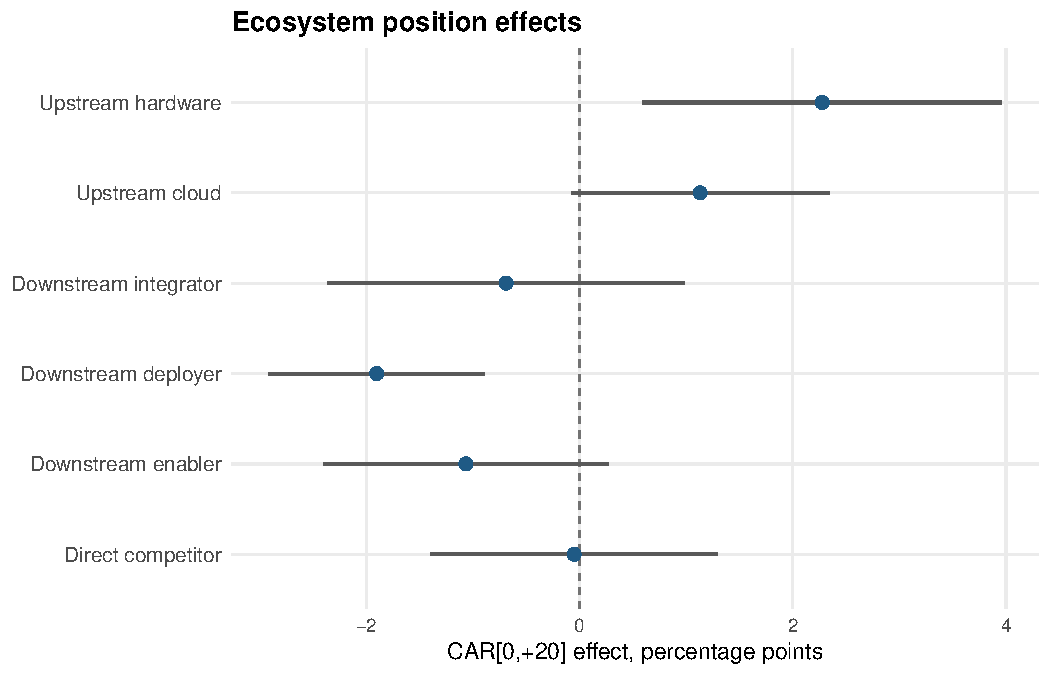
\includegraphics[width=0.88\textwidth]{figure1_position_effects.pdf}
\caption{生态位置效应系数图}
\label{fig:position_effects}
\begin{minipage}{0.9\linewidth}
\vspace{0.3em}
\footnotesize
注：图中报告表~\ref{tab:baseline}中$CAR[0,+20]$窗口的系数估计值，横线为95\%置信区间。上游硬件显著位于零右侧，下游部署显著位于零左侧。
\end{minipage}
\end{figure}

\subsection{合并位置组检验}\label{sec:bundle}

基准表中的六个细分位置验证了异质性的存在，但本文的中心命题，"上游受益、下游受损"，需要一个更直接的检验。表~\ref{tab:bundle}将细分位置合并为上游（$R1\cup R2$）和下游（$R3\cup R4\cup R5$）两大组，直接回答"谁受益、谁受损"这一核心问题。

\begin{table}[H]
\centering
\small
\begin{threeparttable}
\caption{合并位置组效应}
\label{tab:bundle}
\begin{tabular}{lccc}
\toprule
合并位置 & $CAR[0,+10]$ & $CAR[0,+15]$ & $CAR[0,+20]$ \\
\midrule
任意上游（R1$\cup$R2） & 0.82 & 1.80*** & 2.22*** \\
 & (0.53) & (0.67) & (0.78) \\[3pt]
战略上游 & 0.83 & 1.75*** & 2.17*** \\
 & (0.52) & (0.66) & (0.76) \\[3pt]
任意下游（R3$\cup$R4$\cup$R5） & $-$1.22** & $-$2.15*** & $-$2.50*** \\
 & (0.54) & (0.67) & (0.82) \\[3pt]
下游部署（R4） & $-$0.99*** & $-$1.43*** & $-$1.90*** \\
 & (0.36) & (0.43) & (0.51) \\
\midrule
控制变量 & 是 & 是 & 是 \\
年份固定效应 & 是 & 是 & 是 \\
观测值 & 4\,829 & 4\,829 & 4\,829 \\
\bottomrule
\end{tabular}
\begin{tablenotes}
\footnotesize
\item 注：系数单位为百分点。每行为一个独立回归。控制变量和聚类方式同表~\ref{tab:baseline}。*、**、***分别表示在10\%、5\%、1\%水平上显著。$CAR[0,+20]$窗口下，Wild Bootstrap检验中任意上游$p_{wild}<0.001$，任意下游$p_{wild}<0.001$。
\end{tablenotes}
\end{threeparttable}
\end{table}

合并后的结论为假说2提供了更直接的检验。任意上游在$CAR[0,+20]$中为$+2.22$个百分点（$p<0.01$），任意下游为$-2.50$个百分点（$p<0.01$）。一次重大模型发布平均将上下游企业之间的相对估值拉开约4.7个百分点。以2024年末样本企业的平均市值计算，这一差异意味着上游企业群体在单次事件后20个交易日内平均多获得数十亿美元的市值增量，而下游企业群体同步蒸发可比规模的市值。

从产业组织的角度看，这一结果与经典的互补品/替代品分析框架一致。对上游硬件而言，更强的模型意味着更多的训练和推理需求，模型能力与算力是互补关系；对下游部署商而言，更强的模型意味着模型厂商可以直接提供终端功能，应用层的差异化价值被侵蚀，模型能力与下游业务之间呈替代关系。

\subsection{联合回归：控制位置交叠}\label{sec:joint}

前两张表的一个潜在问题是：同一家公司可能同时具有多个位置标签（例如Microsoft既是云服务上游又是竞争者）。若单位置回归的正效应来自与下游位置的负相关，则基准结果可能被高估。表~\ref{tab:joint}将全部六个位置变量同时纳入模型，估计条件于其他位置的净效应。

\begin{table}[H]
\centering
\small
\begin{threeparttable}
\caption{联合位置回归}
\label{tab:joint}
\begin{tabular}{lccc}
\toprule
生态位置 & $CAR[0,+10]$ & $CAR[0,+15]$ & $CAR[0,+20]$ \\
\midrule
上游硬件（R1） & $-$1.35 & $-$0.86 & $-$0.83 \\
 & (1.19) & (1.34) & (1.38) \\[3pt]
上游云服务（R2） & 0.15 & 0.72 & 0.54 \\
 & (0.53) & (0.61) & (0.72) \\[3pt]
下游集成（R3） & $-$1.98* & $-$2.49** & $-$3.09** \\
 & (1.12) & (1.24) & (1.33) \\[3pt]
下游部署（R4） & $-$2.78** & $-$3.41** & $-$4.24*** \\
 & (1.23) & (1.34) & (1.45) \\[3pt]
下游赋能（R5） & $-$2.65*** & $-$3.49*** & $-$3.25*** \\
 & (0.90) & (0.98) & (1.15) \\[3pt]
直接竞争者（R6） & $-$1.24 & $-$1.53* & $-$2.37*** \\
 & (0.79) & (0.82) & (0.87) \\
\midrule
控制变量 & 是 & 是 & 是 \\
年份固定效应 & 是 & 是 & 是 \\
观测值 & 4\,829 & 4\,829 & 4\,829 \\
\bottomrule
\end{tabular}
\begin{tablenotes}
\footnotesize
\item 注：系数单位为百分点。六个位置变量同时进入回归，系数应解读为控制其他位置后的条件净效应。控制变量和聚类方式同表~\ref{tab:baseline}。*、**、***分别表示在10\%、5\%、1\%水平上显著。$CAR[0,+20]$窗口下，Wild Bootstrap检验中上游硬件$p_{wild}=0.61$，下游部署$p_{wild}<0.001$，下游赋能$p_{wild}<0.001$，直接竞争者$p_{wild}=0.02$。
\end{tablenotes}
\end{threeparttable}
\end{table}

联合回归结果需要谨慎解读。上游硬件的系数从单独回归的$+2.28$变为联合回归中的$-0.83$（不显著），这并不意味着上游效应消失，而是反映了严重的多重共线性问题。在本文样本中，上游硬件公司（如NVIDIA）几乎同时出现在每一个事件中，且与多个位置变量高度共线，它们既是硬件供应商，也是模型训练基础设施的直接参与者。当六个相互重叠的虚拟变量同时进入回归时，方差膨胀使得上游系数的估计变得不稳定。本文第五部分的Wild Bootstrap检验进一步确认了这一模式：上游硬件在联合模型中的$p_{wild}=0.61$，而下游部署的$p_{wild}<0.001$。

联合回归还提供了一个关键的稳健性信息：下游三类（集成、部署、赋能）和竞争者在控制位置交叠后\emph{全部}显著为负，且下游部署的系数幅度从单独回归的$-1.90\%$扩大到联合回归的$-4.24\%$。下游的负向效应是整个下游链条的系统性特征，不依赖于模型设定的选择，是本文最稳健的核心发现。

\subsection{开源与闭源异质性}\label{sec:openclose}

前文已确立"上游受益、下游受损"的基准事实。但并非所有模型发布都应当利好上游，关键区别在于模型的开闭源属性。闭源前沿模型只能通过发布者的API获取，其训练和推理高度依赖大规模高端GPU集群，直接巩固算力供应商的需求确定性；而高质量开源模型降低了模型获取门槛，也往往意味着更高的推理效率，同等能力所需算力更少，硬件供应商的边际价值下降。假说3预测，上游硬件溢价应当仅在闭源模型发布中存在，在开源模型发布中消失甚至逆转。表~\ref{tab:openclose}检验这一预测。

\begin{table}[H]
\centering
\small
\begin{threeparttable}
\caption{开源与闭源模型发布的位置效应差异}
\label{tab:openclose}
\begin{tabular}{lccc}
\toprule
生态位置 & 闭源模型 & 开源模型 & 开源$-$闭源 \\
\midrule
上游硬件（R1） & 3.07*** (1.00) & $-$0.59 (1.12) & $-$3.66** (1.50) \\[3pt]
上游云服务（R2） & 1.09 (0.71) & 1.24 (1.76) & 0.15 (2.03) \\[3pt]
下游部署（R4） & $-$2.13*** (0.58) & $-$1.07 (0.93) & 1.06 (1.08) \\[3pt]
下游赋能（R5） & $-$1.29 (0.85) & $-$0.28 (1.27) & 1.01 (1.68) \\[3pt]
直接竞争者（R6） & $-$0.54 (0.83) & 1.73 (1.32) & 2.27 (1.66) \\
\bottomrule
\end{tabular}
\begin{tablenotes}
\footnotesize
\item 注：系数单位为百分点，报告$CAR[0,+20]$窗口。前两列分别为闭源和开源模型发布时的位置效应估计值，第三列为交互项（开源相对于闭源的差异）。括号内为按事件聚类的标准误。控制变量同表~\ref{tab:baseline}。*、**、***分别表示在10\%、5\%、1\%水平上显著。Wild Bootstrap检验中，上游硬件$\times$开源交互项$p_{wild}=0.04$，下游部署$\times$开源交互项$p_{wild}=0.30$。
\end{tablenotes}
\end{threeparttable}
\end{table}

结果精确地验证了假说3。闭源模型发布时，上游硬件企业获得$+3.07$个百分点的异常收益（$p<0.01$）；开源模型发布时，该效应降至$-0.59$个百分点且不显著。交互项为$-3.66$个百分点（$p=0.018$），统计上确认了闭源与开源之间上游效应的显著差异。Wild Bootstrap检验同样支持这一结论（$p_{wild}=0.04$）。在经济意义上，$-3.66$个百分点的交互效应意味着，同样一次模型发布，仅仅因为开源与闭源的区别，上游硬件企业的市场反应就相差约3.7个百分点，以NVIDIA约3万亿美元的市值计算，这一差异对应约1\,100亿美元的估值落差，是DeepSeek R1发布当日NVIDIA实际蒸发市值（5\,900亿美元）的约五分之一。\footnote{$-3.66\%$是全样本平均交互效应，而DeepSeek R1当日$-16.9\%$是单一极端事件的实际跌幅，二者并非同一数量级，不应混同：样本层面的平均效应反映的是系统性规律的稳健下限，个别事件可能因市场情绪放大而显著超过平均水平。}这一发现说明，2025年1月DeepSeek R1引发NVIDIA暴跌并非孤立事件，而是开源高效模型削弱市场对独占式高端算力需求预期这一规律的一次极端体现。

下游方面，闭源模型对部署型下游的负向效应（$-2.13\%$）大于开源模型（$-1.07\%$），方向符合闭源模型更强地约束下游企业获取替代技术的直觉，但交互项（$+1.06\%$, $p=0.33$）未达显著水平。这种不对称的解释力具有经济含义：开闭源的最大区别在于谁获得算力租金，而非谁免于被替代。即便模型开源，下游公司仍面临能力边界扩张带来的竞争压力；开源仅改变了竞争压力的来源，由依赖API的模型提供商转变为任何能够部署开源模型的竞争者。

\begin{figure}[H]
\centering
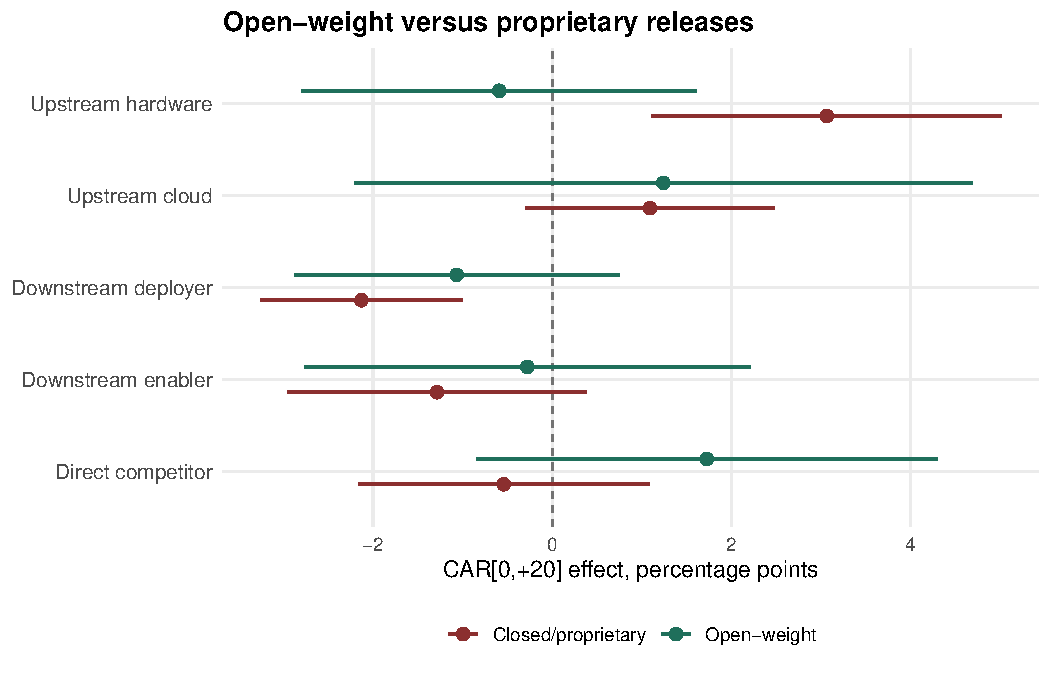
\includegraphics[width=0.88\textwidth]{figure2_open_closed_effects.pdf}
\caption{开源与闭源模型发布的位置效应对比}
\label{fig:open_closed_effects}
\begin{minipage}{0.9\linewidth}
\vspace{0.3em}
\footnotesize
注：图中报告$CAR[0,+20]$窗口下闭源和开源模型发布分别对应的位置效应系数，横线为95\%置信区间。
\end{minipage}
\end{figure}


%% ========================================
\section{稳健性检验}
%% ========================================

为确保核心发现不依赖于特定的样本选择、模型设定或推断方法，本节从四个维度进行系统性的稳健性检验。

\subsection{控制模型能力指标}

一个合理的替代解释是：上游效应可能源于能力更强的模型恰好由与上游企业关联更紧密的发布者发布。为排除这一混淆，本文在基准回归中加入AA Intelligence Index（标准化的模型能力综合评分），将因能力水平差异导致的市场反应从位置效应中剥离。由于AA指标仅覆盖47个事件（3\,780条观测），该规格作为稳健性补充报告。

\begin{table}[H]
\centering
\small
\begin{threeparttable}
\caption{控制模型能力指标后的位置效应}
\label{tab:aa_control}
\begin{tabular}{lccc}
\toprule
生态位置 & $CAR[0,+10]$ & $CAR[0,+15]$ & $CAR[0,+20]$ \\
\midrule
上游硬件（R1） & 1.15* & 2.26** & 3.05*** \\
 & (0.67) & (0.86) & (0.97) \\[3pt]
任意上游 & 1.27** & 2.30*** & 2.87*** \\
 & (0.60) & (0.77) & (0.90) \\[3pt]
任意下游 & $-$1.86*** & $-$2.82*** & $-$3.30*** \\
 & (0.57) & (0.70) & (0.87) \\[3pt]
下游部署（R4） & $-$1.00** & $-$1.58*** & $-$2.02*** \\
 & (0.42) & (0.50) & (0.54) \\
\midrule
AA Intelligence控制 & 是 & 是 & 是 \\
控制变量 & 是 & 是 & 是 \\
年份固定效应 & 是 & 是 & 是 \\
观测值 & 3\,780 & 3\,780 & 3\,780 \\
\bottomrule
\end{tabular}
\begin{tablenotes}
\footnotesize
\item 注：系数单位为百分点。每行为一个独立回归。所有模型额外控制AA Intelligence Index（标准化的模型能力综合评分），AA指标仅覆盖47个事件，故样本缩减至3\,780条观测。其余控制变量同表~\ref{tab:baseline}。*、**、***分别表示在10\%、5\%、1\%水平上显著。
\end{tablenotes}
\end{threeparttable}
\end{table}

表~\ref{tab:aa_control}显示，控制能力指标后，位置效应不仅方向不变，幅度还有所增大：上游硬件$CAR[0,+20]=+3.05\%$（较基准$+2.28\%$增大34\%），下游部署$=-2.02\%$（较基准$-1.90\%$增大6\%）。这表明，在前文基准回归中，能力变异实际上略微掩盖了位置效应，能力较强的模型同时吸引了更多"全行业利好"预期，从而部分对冲了位置方向性的效应。剥离能力成分后，位置再定价的信号更加清晰。

\subsection{上游硬件与云服务差异的正式检验}

基准回归显示上游硬件（$+2.28\%$）的点估计高于上游云服务（$+1.13\%$），直觉上似乎上游效应主要由硬件驱动。为正式检验这一印象，本文将两个上游变量同时纳入回归并进行Wald差异检验，结果见表~\ref{tab:r1_diff}。

\begin{table}[H]
\centering
\small
\begin{threeparttable}
\caption{上游硬件与云服务系数差异的Wald检验}
\label{tab:r1_diff}
\begin{tabular}{lcccccc}
\toprule
窗口 & $\hat{\beta}_{\text{硬件}}$ & $\hat{\beta}_{\text{云服务}}$ & 差异 & $SE_{\text{差异}}$ & $z$ & $p$ \\
\midrule
$CAR[0,+10]$ & 0.75 & 1.12 & $-$0.37 & 0.67 & $-$0.553 & 0.580 \\
$CAR[0,+15]$ & 1.76 & 1.97 & $-$0.20 & 0.71 & $-$0.285 & 0.776 \\
$CAR[0,+20]$ & 2.37 & 1.61 & 0.76 & 0.73 & 1.040 & 0.298 \\
\bottomrule
\end{tabular}
\begin{tablenotes}
\footnotesize
\item 注：系数单位为百分点。两个上游变量同时进入回归，对$\hat{\beta}_{\text{硬件}}-\hat{\beta}_{\text{云服务}}$进行Wald检验。$n=4\,829$，60个事件聚类。控制变量同表~\ref{tab:baseline}。
\end{tablenotes}
\end{threeparttable}
\end{table}

三个窗口的差异检验均不显著（$p$值分别为0.580、0.776、0.298）。硬件和云服务的点估计方向一致（均为正），$CAR[0,+20]$窗口下硬件略大于云服务，但两者在统计上不可区分。本文据此认为，上游正向效应是硬件和云服务的共同特征，两者在当前样本量下无法显著区分，不将"上游效应主要由硬件驱动"作为经过正式检验确认的结论。

\subsection{核心变量全窗口全方法稳健性}

下游部署（R4）是本文证据强度最高的核心发现。为验证其稳健性不依赖于特定窗口选择或推断方法，表~\ref{tab:r2_robust}报告该变量在全部7个CAR窗口下的系数、以及三种推断方法（CR0、CR2、Wild Bootstrap）的$p$值。

\begin{table}[H]
\centering
\small
\begin{threeparttable}
\caption{下游部署效应的全窗口全方法稳健性}
\label{tab:r2_robust}
\begin{tabular}{lcccccc}
\toprule
窗口 & $\hat{\beta}$（百分点） & $SE$ & $n$ & $p_{CR0}$ & $p_{CR2}$ & $p_{wild}$ \\
\midrule
$CAR[0,+1]$ & $-$0.34 & 0.14 & 4\,809 & 0.018 & 0.020 & 0.020 \\
$CAR[0,+2]$ & $-$0.42 & 0.18 & 4\,815 & 0.019 & 0.021 & 0.022 \\
$CAR[0,+3]$ & $-$0.53 & 0.20 & 4\,823 & 0.009 & 0.010 & 0.009 \\
$CAR[0,+5]$ & $-$0.72 & 0.24 & 4\,826 & 0.004 & 0.005 & 0.002 \\
$CAR[0,+10]$ & $-$0.99 & 0.36 & 4\,829 & 0.008 & 0.008 & 0.007 \\
$CAR[0,+15]$ & $-$1.43 & 0.43 & 4\,829 & 0.002 & 0.002 & 0.001 \\
$CAR[0,+20]$ & $-$1.90 & 0.51 & 4\,829 & 0.0004 & 0.0005 & 0.0004 \\
\bottomrule
\end{tabular}
\begin{tablenotes}
\footnotesize
\item 注：每行为一个独立回归，仅含下游部署（R4）虚拟变量。Wild Bootstrap采用Rademacher权重，$B=4\,999$次，施加零假设约束。控制变量同表~\ref{tab:baseline}。
\end{tablenotes}
\end{threeparttable}
\end{table}

结果呈现出三个显著特征。第一，效应方向在全部7个窗口一致为负，从事件日后第1个交易日的$-0.34$个百分点单调增长至第20个交易日的$-1.90$个百分点（约5.7倍），显著性同步增强。这种效应随时间推移逐步增强的模式更符合渐进信息扩散和重新定价的解释，而非公告日一次性超调后反转的解释。第二，三种推断方法在每个窗口高度一致（$p$值彼此差异不超过0.002），且从未出现一种方法显著而另一种方法不显著的情况。第三，在60个事件聚类这一中等聚类数下，Wild Bootstrap与渐近方法的高度吻合本身即构成有意义的推断稳健性证据。

将Wild Bootstrap检验扩展到表~\ref{tab:baseline}、表~\ref{tab:bundle}、表~\ref{tab:joint}和表~\ref{tab:openclose}的核心系数后，可以看到下游部署效应在基准、合并组、联合回归、开闭源交互四种模型设定下均高度显著（$p_{wild}<0.001$至$0.02$），是本文唯一在全部设定下都通过检验的系数；上游硬件在前三种设定下稳健（$p_{wild}=0.02$至$0.04$），但在联合回归中失去显著性（$p_{wild}=0.61$，对应第\ref{sec:joint}节讨论的多重共线性问题）。

\subsection{剔除极端事件与逐一剔除分析}

一个常见的质疑是核心发现可能由少数极端观测驱动。为此，本文进行三项敏感性检验：（1）剔除DeepSeek R1事件（2025年1月发布，引发NVIDIA单日暴跌的极端事件）后重估；（2）逐一剔除60个事件（leave-one-event-out）；（3）逐一剔除86家公司（leave-one-firm-out）。结果见表~\ref{tab:r3_sensitivity}。

\begin{table}[H]
\centering
\small
\begin{threeparttable}
\caption{极端事件与逐一剔除敏感性分析（$CAR[0,+20]$）}
\label{tab:r3_sensitivity}
\begin{tabular}{lcc}
\toprule
 & 上游硬件（R1） & 下游部署（R4） \\
\midrule
\multicolumn{3}{l}{\textit{面板A：剔除DeepSeek R1}} \\
\quad 全样本基准 & 2.28*** (0.84) & $-$1.90*** (0.51) \\
\quad 剔除后 & 2.28*** (0.86) & $-$1.86*** (0.51) \\
\quad 系数变化幅度 & 0.2\% & 2.2\% \\[6pt]
\multicolumn{3}{l}{\textit{面板B：逐一剔除事件（60次迭代）}} \\
\quad 系数范围 & [2.03, 2.49] & [$-$2.04, $-$1.74] \\
\quad 系数标准差 & 0.111 & 0.067 \\
\quad 最大影响事件 & FMR-0056 & FMR-0016 \\
\quad 符号翻转次数 & 0/60 & 0/60 \\
\quad 失去10\%显著性次数 & 0/60 & 0/60 \\[6pt]
\multicolumn{3}{l}{\textit{面板C：逐一剔除公司（86次迭代）}} \\
\quad 系数范围 & [2.04, 2.49] & [$-$2.08, $-$1.68] \\
\quad 系数标准差 & 0.076 & 0.065 \\
\quad 最大影响公司 & SMCI & 5803 JP \\
\quad 符号翻转次数 & 0/86 & 0/86 \\
\quad 失去10\%显著性次数 & 0/86 & 0/86 \\
\bottomrule
\end{tabular}
\begin{tablenotes}
\footnotesize
\item 注：面板A报告剔除DeepSeek R1事件前后的系数对比。面板B和C分别报告逐一剔除事件和公司后的系数分布统计量。"最大影响事件/公司"指剔除后系数偏离全样本估计最大的观测。括号内为按事件聚类的标准误。*、**、***分别表示在10\%、5\%、1\%水平上显著。
\end{tablenotes}
\end{threeparttable}
\end{table}

结果表明，两个核心发现均不由单一事件或单一公司驱动。DeepSeek R1的剔除对系数几乎没有影响（上游硬件变化0.2\%，下游部署变化2.2\%）。在全部60次逐一剔除事件和86次逐一剔除公司的迭代中，两个核心变量均未出现符号翻转或显著性丧失。下游部署的稳定性尤为突出，其系数的标准差仅为0.067个百分点，说明这一发现高度均匀地分布在整个样本中，不存在关键驱动观测。此外，将样本按DeepSeek R1事件日（2025年1月22日）一分为二分别重新估计基准位置效应，上游硬件效应在前后两个子样本中方向一致（前20次发布$+2.27\%$，后40次发布$+2.18\%$，均为正），下游部署效应在两个子样本中均显著为负（前20次$-3.14\%$，$p<0.01$；后40次$-1.11\%$，$p<0.05$），说明本文记录的位置异质性并非由DeepSeek R1这一单一极端事件事后定义出来的模式，而是在该事件发生之前就已经存在的规律。\footnote{该子样本拆分回归的完整结果保存在补充材料中，因不改变本节结论的方向性，正文不再单列表格。}



%% ========================================
\section{进一步分析与机制讨论}
%% ========================================

\subsection{为何只有下游部署型（R4）显著为负}

基准回归中，三类下游位置的效应存在明显层级差异：下游部署（R4）在所有窗口显著为负，下游赋能（R5）在部分窗口显著，而下游集成（R3）在单独回归中不显著。这一差异具有清晰的经济解释。

下游部署型企业（R4）是将AI作为工具嵌入传统业务的公司，其核心竞争力不在于AI技术本身，而在于传统业务的客户关系、行业know-how和运营能力。当前沿模型能力大幅跃升时，模型发布方可以直接向终端用户提供这些企业原本提供的功能（如文档生成、客服自动化、数据分析），其差异化价值面临最直接的侵蚀。

相比之下，下游集成型企业（R3）的核心业务本身就是围绕AI展开的，它们是AI原生的，其竞争力在于如何更好地利用最新模型。对这类企业而言，新模型的发布既是威胁（旧的集成方案可能过时）也是机遇（可以利用更强的模型构建更好的产品），两者部分对冲，导致净效应不明确。下游赋能型企业（R5，IT咨询/外包）则处于中间，AI能力提升既增加了企业对AI咨询的需求（正面），也使得部分基础咨询工作可被模型直接替代（负面）。

联合回归进一步支持了这一解释：当控制位置交叠后，R3的系数变为显著负向（$-3.09\%$，$p<0.05$），说明在单位置回归中，R3企业的正面机遇效应被同时具有的其他身份（如竞争者）所混淆；一旦净化这种混淆，下游集成的"被替代"效应也显现出来。

\subsection{开闭源调节的经济机制}

表~\ref{tab:openclose}显示开闭源属性显著调节上游效应但不显著调节下游效应，这一不对称性反映了开闭源之间的核心区别在于算力租金的归属，而不在于替代威胁的有无。

具体而言：（1）闭源模型由少数拥有大规模GPU集群的实验室独占运营，其部署需要集中的推理算力，直接巩固硬件供应商的垄断地位和需求确定性；（2）开源模型允许任何人本地部署或使用更小规模的推理方案，同等能力所需算力更分散、单位GPU边际价值下降，硬件供应商的独占性租金被稀释。

但对下游而言，无论模型是开源还是闭源，其能力边界的扩张都意味着传统应用层的差异化价值被侵蚀，开源仅改变了竞争压力的来源，由依赖API的模型提供商转变为任何能够部署开源模型的竞争者。开闭源属性不显著调节下游负向效应符合这一经济逻辑，而非检验力不足导致的偶然结果。

\subsection{推理模型与代码模型的算力强度信号}\label{sec:reasoning_code_het}

开闭源属性调节的是算力租金的归属，即谁能从模型发布中获得对独占式算力的需求确认。模型本身的技术形态也可能独立地调节市场对算力消耗密度的预期，而无需借助开闭源这一渠道。本节考察两类直接指向算力强度的模型特征，推理能力与代码生成能力，分别对应推理时算力（test-time compute）和训练/工具链算力两条不同的算力需求路径。两项检验均沿用表~\ref{tab:baseline}的回归设定，控制变量、按事件聚类的稳健标准误，结果见表~\ref{tab:het_reasoning_code}与图~\ref{fig:reasoning_code_effects}。

本文样本中17次发布包含具备链式推理能力的模型，如OpenAI o1/o3系列、DeepSeek R1。表~\ref{tab:het_reasoning_code}面板A显示，当发布事件包含推理模型时，上游硬件的$CAR[0,+20]$效应从非推理模型发布时的$+1.61\%$（不显著）上升至$+3.96\%$（$p<0.01$），交互项为$+2.35\%$（$p=0.173$，未达统计显著）。下游部署的负向效应同样在推理模型发布时有所放大，从$-1.67\%$到$-2.47\%$，但交互项不显著（$p=0.522$）。这一模式符合直觉：推理模型在推理阶段需要消耗远超传统模型的算力，因而更直接地强化市场对算力需求的预期；交互项未达统计显著可能与推理模型发布数量较少（仅17次）带来的检验力限制有关。

为检验上述算力强度信号逻辑是否具有一般性，本文进一步考察代码模型（专门面向代码生成与补全场景的模型，本文样本中16次发布属于此类）的调节作用。如果代码模型与推理模型一样主要通过提升算力消耗密度来强化上游溢价，理论上应观察到类似的正向交互，但表~\ref{tab:het_reasoning_code}面板B显示了相反的模式。非代码模型发布时上游硬件效应为$+2.97\%$（$p<0.01$），代码模型发布时降至$+0.35\%$（不显著），交互项为$-2.63\%$（$p=0.151$，未达统计显著但方向与推理模型相反）；下游部署效应在两类发布中差异很小，$-1.93\%$对$-1.81\%$，交互项$p=0.891$。模型技术形态并不是一个能一概而论地强化上游溢价的单一维度。推理模型直接对应可观测、可预期的额外算力消耗，每次查询的推理时长与算力成本随链式推理步数上升，代码模型的算力需求则更多体现在训练阶段和工具链集成上，发布时点本身未必传递同等强度的新增算力需求信号。代码模型发布也更可能被市场理解为产品功能扩展而非算力规模信号，二者对市场预期形成的渠道有本质区别。

两项交互检验均未达到统计显著（推理模型$p=0.173$，代码模型$p=0.151$），样本量较小（17/43、16/44）限制了检验力，但代码模型方向相反这一发现本身具有信息量：它提示不能简单地用是否为前沿技术亮点作为算力强度的代理变量，而应聚焦于该技术特征是否直接对应可预期的、增量的训练或推理算力消耗。

\begin{table}[H]
\centering
\small
\begin{threeparttable}
\caption{推理模型与代码模型的交互效应（$CAR[0,+20]$）}
\label{tab:het_reasoning_code}
\begin{tabular}{lccc}
\toprule
 & 上游硬件 & 任意上游 & 下游部署 \\
\midrule
\multicolumn{4}{l}{\textit{面板A：推理模型交互（17次推理模型发布 vs. 43次非推理模型发布）}} \\
非推理模型发布 & 1.61 (1.00) & 1.49 (0.94) & $-$1.67*** (0.57) \\
推理模型发布 & 3.96*** (1.43) & 4.05*** (1.37) & $-$2.47** (1.09) \\
交互项（推理$-$非推理） & 2.35 (1.72) & 2.56 (1.68) & $-$0.80 (1.25) \\[4pt]
\multicolumn{4}{l}{\textit{面板B：代码模型交互（16次代码模型发布 vs. 44次非代码模型发布）}} \\
非代码模型发布 & 2.97*** (0.97) & 2.86*** (0.90) & $-$1.93*** (0.63) \\
代码模型发布 & 0.35 (1.57) & 0.47 (1.61) & $-$1.81*** (0.70) \\
交互项（代码$-$非代码） & $-$2.63 (1.83) & $-$2.39 (1.88) & 0.13 (0.93) \\
\bottomrule
\end{tabular}
\begin{tablenotes}
\footnotesize
\item 注：系数单位为百分点，$n=4\,829$，60个事件聚类。两个面板各为一组独立交互回归，"交互项"为调节变量取值从0变为1时的位置效应差异，括号内为按事件聚类的稳健标准误。控制变量同表~\ref{tab:baseline}。*、**、***分别表示在10\%、5\%、1\%水平上显著。
\end{tablenotes}
\end{threeparttable}
\end{table}

\begin{figure}[H]
\centering
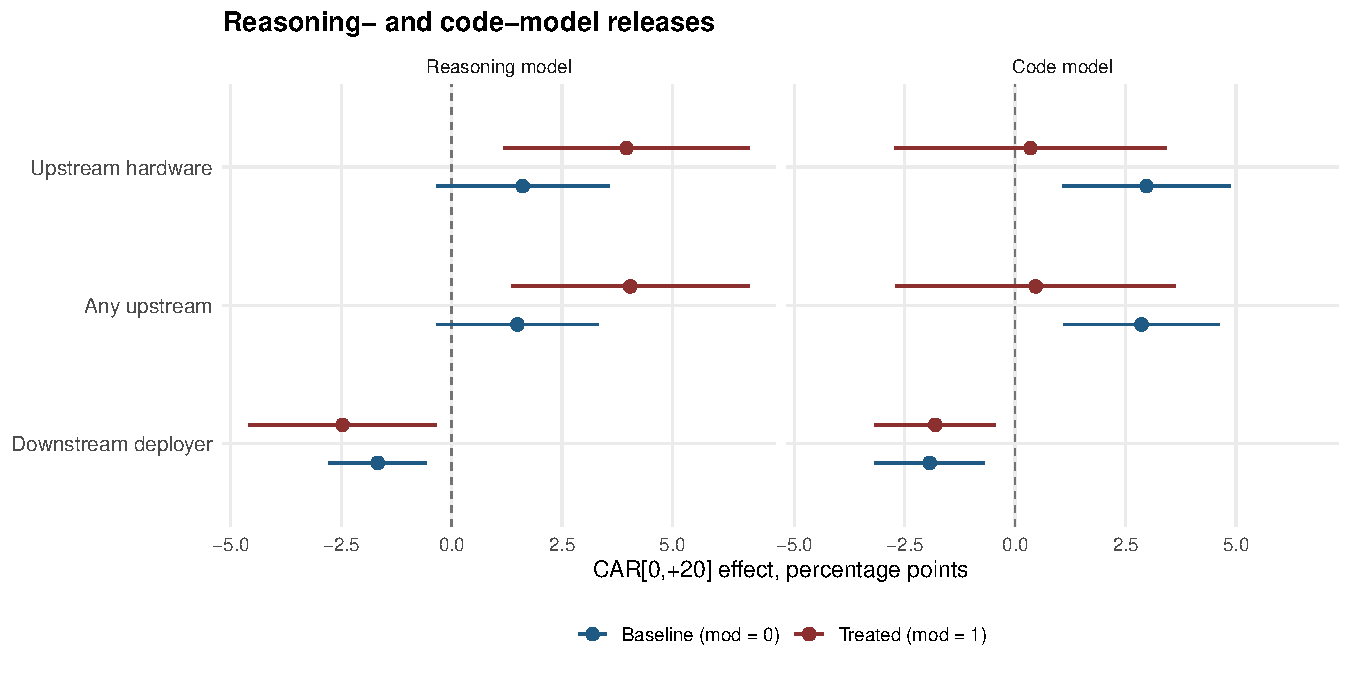
\includegraphics[width=0.95\textwidth]{figure3_reasoning_code_effects.pdf}
\caption{推理模型与代码模型发布的位置效应对比}
\label{fig:reasoning_code_effects}
\begin{minipage}{0.92\linewidth}
\vspace{0.3em}
\footnotesize
注：图中报告$CAR[0,+20]$窗口下推理模型（左）与代码模型（右）发布的位置效应系数，横线为95\%置信区间。蓝色为调节变量取0时（非推理/非代码模型发布）的效应，红色为调节变量取1时（推理/代码模型发布）的效应。
\end{minipage}
\end{figure}

\subsection{模型发布方来源国的调节效应及其共线性结构}\label{sec:origin_het}

本文样本中13次发布由中国厂商主导（如DeepSeek、阿里、智谱等），其余47次由美国及其他国家厂商发布。这一来源国划分揭示了本文全部交互检验中统计上最强的一个调节效应，但其背后的共线性结构也最为复杂，值得展开讨论。结果见表~\ref{tab:het_origin}与图~\ref{fig:origin_effects}。

表~\ref{tab:het_origin}面板A显示，非中国厂商发布时上游硬件获得$+3.38\%$的显著正向效应（$p<0.01$），而中国厂商发布时该效应转为$-1.80\%$（不显著），交互项为$-5.18\%$（$p<0.01$），统计上高度显著，且方向与幅度均强于开闭源交互项本身（$-3.66\%$，见表~\ref{tab:openclose}）。原因在于本文样本中的中国厂商发布几乎全部为开源或开放权重模型：13次中国厂商发布中8次为开源，相较于47次非中国厂商发布中仅5次为开源，占比62\%对11\%。中国厂商发布因此同时承载了开源属性与训练效率叙事两层信号，DeepSeek R1以远低于行业旗舰模型的训练成本达到可比性能，这一叙事本身强化了市场对算力需求确定性下降的预期，对上游硬件溢价的冲击力度因此超过单纯的开源效应。

上述效应是否真的反映中国厂商这一地理属性，还是更可能由一个相关但本质不同的因素驱动，例如中国厂商在样本期内更可能以未上市新创公司或国有研究机构身份发布，缺乏覆盖面广的分析师网络和做市深度，导致市场对其发布的预期形成路径本就与已上市成熟企业不同，这是一个值得检验的问题。为此，本文构造发布方是否为上市公司这一变量，涵盖美股上市公司及其他国家的上市公司，重新估计同样的交互模型。表~\ref{tab:het_origin}面板B显示，上市发布方与非上市发布方的上游硬件效应几乎没有差异，分别为$+2.31\%$和$+2.24\%$，交互项仅$+0.07\%$（$p=0.967$）。这一结果排除了上市状态这一替代解释，说明来源国效应并非由资本市场结构性因素驱动，而与中国厂商发布所携带的开源属性和效率叙事复合信号直接相关。

第三步，本文同时把开闭源交互项与来源国交互项纳入同一回归，检验来源国效应在多大程度上独立于开源效应。表~\ref{tab:het_origin}面板C显示，在联合模型中，$upstream\_hardware \times is\_open\_weight$交互项的点估计为$-1.42\%$且不显著（$p=0.478$），而$upstream\_hardware \times is\_chinese\_model$交互项仍为$-4.45\%$且在5\%水平上显著（$p=0.021$）。当开源属性和来源国同时进入回归、相互竞争对上游溢价的解释力时，来源国交互项保留了统计显著性，开源交互项的点估计反而被压缩并失去显著性。来源国变量捕捉到的信息比单纯的是否开源更丰富，可能同时承载了效率叙事、地缘政治预期调整等开源属性之外的成分。样本中开源与中国厂商高度相关（8/13对5/47），联合模型中两个交互项的标准误均有所放大，属于预期之内的估计精度损失。\footnote{来源国效应是否部分由西方财经媒体对中国厂商发布的报道基调系统性更负面所驱动，这一传导渠道在下一节中作单独检验。}

综合以上三步，模型来源国是本文证据等级最高的调节效应之一，但其解释需放在开源属性和效率叙事的联合背景下理解，不宜简化为单一的地理政治叙事；发布方上市状态的零结果为排除资本市场结构性替代解释提供了证据。

\begin{table}[H]
\centering
\small
\begin{threeparttable}
\caption{模型发布方来源国的调节效应及其共线性诊断（$CAR[0,+20]$）}
\label{tab:het_origin}
\begin{tabular}{lccc}
\toprule
 & 上游硬件 & 任意上游 & 任意下游 \\
\midrule
\multicolumn{4}{l}{\textit{面板A：模型来源国交互（13次中国厂商发布 vs. 47次非中国厂商发布）}} \\
非中国厂商发布 & 3.38*** (0.97) & 3.11*** (0.92) & $-$3.19*** (0.91) \\
中国厂商发布 & $-$1.80 (1.13) & $-$1.08 (1.26) & 0.09 (1.71) \\
交互项（中国$-$非中国） & $-$5.18*** (1.50) & $-$4.19*** (1.62) & 3.28* (1.95) \\[4pt]
\multicolumn{4}{l}{\textit{面板B：发布方上市状态交互（共线性诊断，30次上市发布方 vs. 30次非上市发布方）}} \\
非上市发布方 & 2.24* (1.21) & 2.02* (1.16) & $-$1.95 (1.26) \\
上市发布方 & 2.31** (1.13) & 2.43** (1.07) & $-$3.04*** (1.01) \\
交互项（上市$-$非上市） & 0.07 (1.63) & 0.41 (1.59) & $-$1.10 (1.59) \\[4pt]
\multicolumn{4}{l}{\textit{面板C：开源$\times$来源国联合模型（同时纳入两个交互项）}} \\
位置主效应 & 3.53*** (0.99) & 3.26*** (0.94) & --- \\
$\times$开源（交互项） & $-$1.42 (1.98) & $-$1.40 (2.04) & --- \\
$\times$中国厂商（交互项） & $-$4.45** (1.88) & $-$3.48* (1.91) & --- \\
\bottomrule
\end{tabular}
\begin{tablenotes}
\footnotesize
\item 注：系数单位为百分点，$n=4\,829$，60个事件聚类。面板A、B的"交互项"为调节变量取值从0变为1时的位置效应差异。面板C为联合回归，同时纳入位置变量与开源、来源国两个调节变量及其交互项，控制变量与位置主效应一并估计；下游列因联合模型仅聚焦上游变量未予报告。括号内为按事件聚类的稳健标准误。控制变量同表~\ref{tab:baseline}。*、**、***分别表示在10\%、5\%、1\%水平上显著。
\end{tablenotes}
\end{threeparttable}
\end{table}

\begin{figure}[H]
\centering
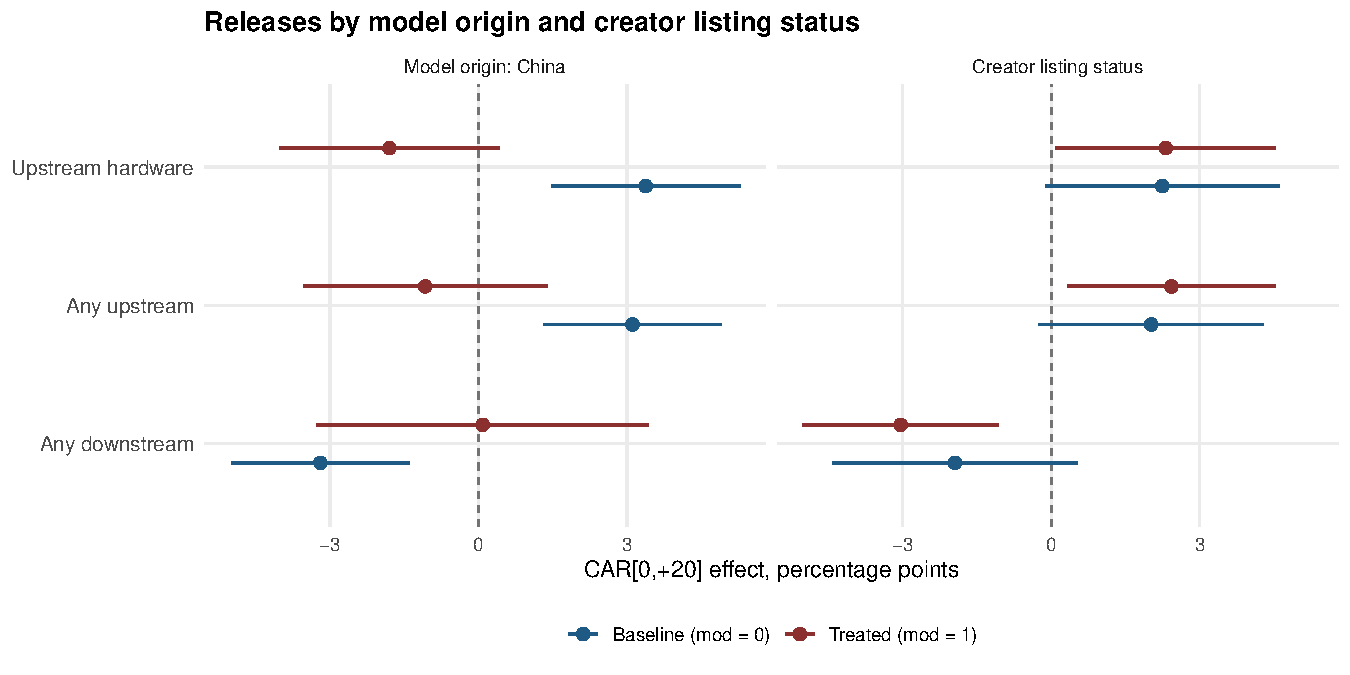
\includegraphics[width=0.95\textwidth]{figure4_origin_effects.pdf}
\caption{模型来源国与发布方上市状态的位置效应对比}
\label{fig:origin_effects}
\begin{minipage}{0.92\linewidth}
\vspace{0.3em}
\footnotesize
注：图中报告$CAR[0,+20]$窗口下模型来源国（左）与发布方上市状态（右）的位置效应系数，横线为95\%置信区间。左图蓝色为非中国厂商发布、红色为中国厂商发布；右图蓝色为非上市发布方、红色为上市发布方。右图两组效应高度重叠，与左图的方向分化形成对照。
\end{minipage}
\end{figure}

\subsection{媒体关注度的调节作用}\label{sec:media_het}

前两节考察的是事件本身的技术或来源属性，本节考察模型发布后的媒体报道基调是否系统性调节位置效应的大小。这一检验对应上一节提出的问题，即来源国效应是否部分由西方财经媒体对中国厂商发布的报道基调更负面所驱动。

本文使用事件层面$[0,+20]$窗口内的媒体报道情绪均值（取值范围约$-0.11$至$+0.55$，越高表示报道基调越正面）作为调节变量，覆盖60次发布事件中的54次。为便于解释，本文将该变量标准化为z-score后与位置变量构造连续交互项，回归设定与表~\ref{tab:baseline}一致，结果见表~\ref{tab:het_media}与图~\ref{fig:media_sentiment_effects}。

交互项本身在四个位置变量上均不显著，上游硬件$p=0.853$，任意上游$p=0.322$，任意下游$p=0.526$，下游部署$p=0.586$，且四个交互项的点估计量级都很小，介于$+0.17$至$+0.79$个百分点之间，相对于位置主效应2至3个百分点的量级并不大。图~\ref{fig:media_sentiment_effects}显示，媒体情绪从$-1$个标准差移动到$+1$个标准差时，四类位置效应的点估计几乎平行移动，置信区间高度重叠。这说明媒体情绪不是来源国效应背后的中介渠道，来源国效应更可能直接来自开源属性与效率叙事这一复合信号。

控制位置变量后，媒体情绪的主效应在四个模型中均为负，约$-0.8$至$-1.4$个百分点每标准差，其中上游硬件、任意上游、下游部署三个模型中达到10\%或5\%水平显著。报道基调更正面的发布事件，整体$CAR[0,+20]$反而略低，方向与"报道越积极、市场反应越正面"的朴素预期相反。这可能与反向因果有关：媒体报道基调或许是对模型发布是否符合预期的事后总结，如果一次发布的市场反应在公告日已经迅速消化、后续超额收益空间有限，相关报道反而可能呈现更积极的基调；需要更长时间被市场重新定价的意外性事件，报道基调可能更具保留态度，事后却伴随更大的累计异常收益。本文的样本量和检验设计无法区分这一解释与其他可能机制，这一发现是一个描述性模式，有待后续研究检验。

\begin{table}[H]
\centering
\small
\begin{threeparttable}
\caption{媒体情绪的连续交互效应（$CAR[0,+20]$）}
\label{tab:het_media}
\begin{tabular}{lcccc}
\toprule
 & 上游硬件 & 任意上游 & 任意下游 & 下游部署 \\
\midrule
位置主效应（情绪取均值） & 2.80*** (0.91) & 2.76*** (0.84) & $-$2.90*** (0.89) & $-$1.84*** (0.56) \\
情绪主效应（每1标准差） & $-$1.22** (0.56) & $-$1.41** (0.58) & $-$0.79 (0.58) & $-$1.21*** (0.46) \\
交互项（位置$\times$情绪） & 0.17 (0.90) & 0.79 (0.80) & $-$0.59 (0.93) & 0.20 (0.36) \\
情绪$-1$标准差时的位置效应 & 2.64** (1.29) & 1.97* (1.11) & $-$2.32 (1.44) & $-$2.04*** (0.76) \\
情绪$+1$标准差时的位置效应 & 2.97** (1.26) & 3.55*** (1.21) & $-$3.49*** (1.11) & $-$1.65*** (0.55) \\
\bottomrule
\end{tabular}
\begin{tablenotes}
\footnotesize
\item 注：系数单位为百分点，$n=4\,198$，54个事件聚类（媒体情绪数据覆盖60次事件中的54次）。媒体情绪为事件层面$[0,+20]$窗口媒体报道情绪均值的标准化值（z-score）。控制变量同表~\ref{tab:baseline}。括号内为按事件聚类的稳健标准误。*、**、***分别表示在10\%、5\%、1\%水平上显著。
\end{tablenotes}
\end{threeparttable}
\end{table}

\begin{figure}[H]
\centering
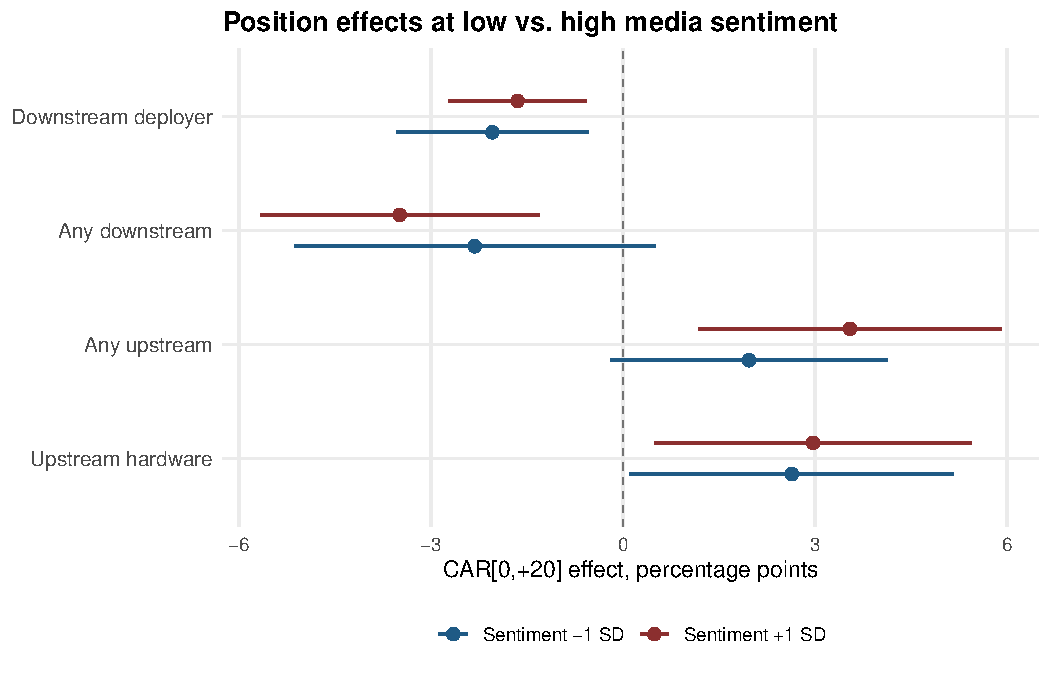
\includegraphics[width=0.88\textwidth]{figure5_media_sentiment_effects.pdf}
\caption{低媒体情绪与高媒体情绪下的位置效应对比}
\label{fig:media_sentiment_effects}
\begin{minipage}{0.9\linewidth}
\vspace{0.3em}
\footnotesize
注：图中报告$CAR[0,+20]$窗口下媒体情绪取$-1$个标准差（蓝色）与$+1$个标准差（红色）时的位置效应系数，横线为95\%置信区间。四组对比中置信区间高度重叠，表明媒体情绪对位置效应的调节作用较弱。
\end{minipage}
\end{figure}

\subsection{上游硬件效应的证据强度评估}

综合本文全部实证检验，上游硬件正效应的证据状况如下：

\begin{enumerate}[leftmargin=2em]
\item 方向性稳健：在基准回归、合并组、控制能力指标、逐一剔除等设定下，系数始终为正且显著（$p_{wild}=0.02$）。
\item 经济机制清晰：闭源$+3.07\%$、开源$-0.59\%$的对比与算力互补/替代理论完全一致。
\item 设定敏感性：在联合回归中（6个高度共线的位置变量同时进入），系数翻转为负且完全不显著（$p_{wild}=0.61$）。
\item 与云服务不可区分：Wald差异检验$p=0.298$，无法确认硬件效应独立于更广义的上游效应。
\end{enumerate}

这一证据格局表明，上游正效应是真实的、具有明确经济机制支撑的发现，但它在统计上不是一个可分离的独立效应：更准确的表述是"广义上游位置"（包含硬件和云服务）在模型发布后获得正向重估。


%% ========================================
\section{结论}
%% ========================================

本文以2024--2026年60次重大AI模型发布事件为准自然实验，基于86家美股上市公司的5\,160条事件--公司层面观测，系统性地考察了大语言模型发布沿AI产业链生态位置产生的异质性资本市场反应。研究发现可以凝练为以下三个层次：

第一，位置再定价效应（假说1、假说2）。模型发布沿生态位置产生方向相反的价值再分配。上游硬件企业在事件后20个交易日内平均获得$+2$--$3\%$的累计异常收益，部署型下游企业平均损失约$-2\%$，上下游差异约4--5个百分点。以样本期间上下游企业的平均市值计算，这一差异意味着每一次重大模型发布在20个交易日内引发了上下游之间约80亿美元的相对市值再分配。\footnote{粗略估算：上游硬件企业平均市值约2\,800亿美元$\times 2.28\%\approx$64亿美元；下游部署型企业平均市值约850亿美元$\times 1.90\%\approx$16亿美元；合计约80亿美元的相对再分配。}下游部署效应在全部7个事件窗口（$CAR[0,+1]$至$CAR[0,+20]$）、3种推断方法（CR0、CR2、Wild Bootstrap）、4种模型设定（单位置基准、合并组、联合回归、开闭源交互）下均高度显著，是本文证据强度最高、最无争议的核心发现。

第二，开源调节效应（假说3）。上游溢价仅在闭源模型发布中成立（$+3.07\%$），开源模型发布时该溢价消失甚至逆转（$-0.59\%$），交互项统计显著（$p=0.018$，$p_{wild}=0.04$）。这一发现的机制在于，闭源模型巩固了对独占式高端算力的需求预期，而开源模型通过降低推理门槛和分散算力需求，削弱了硬件供应商的垄断租金。开闭源属性不显著调节下游负向效应（交互项$p=0.30$），表明开闭源之间的核心区别在于算力租金的归属结构，而非替代威胁的有无，这一结果同样具有理论价值。

第三，位置效应独立于模型能力。控制AA Intelligence Index（模型技术能力的标准化综合评分）后，上下游系数不变甚至增大（上游硬件从$+2.28\%$增至$+3.05\%$，下游部署从$-1.90\%$增至$-2.02\%$），说明生态位置是一个独立于技术特征的市场定价维度，企业在产业链中所处的位置本身构成市场重新定价所依据的信息，并不完全由模型能力的强弱决定。

本文的发现对理论发展和政策制定均有一定的启示意义。在理论层面，本文的实证证据为产业组织中经典的互补品/替代品分析框架在技术冲击情境下的适用性提供了新的支持，并揭示了开源/闭源技术路径选择作为产业链外溢效应调节变量的重要作用。在政策层面，研究结果指向AI产业链利润分配结构中的两个关键特征：其一，在闭源技术体制下，模型发布驱动的价值增量高度向算力上游集中，可能加剧产业链内部的收入不平等和市场集中度；其二，开源模型的出现虽然削弱了算力租金向上游集中的程度，但并不自动解决下游企业被替代的问题，下游企业的转型压力源于模型能力边界扩张本身，与开闭源属性无关，是一种结构性挑战而非技术路径选择可以化解的短期冲击。这一发现对于AI产业政策的制定，特别是关于开源激励、算力基础设施布局和下游企业转型支持，具有参考价值。

本文发现的证据强度存在不对称性，并存在若干局限性。下游部署效应具有无条件稳健性，可以不附带限定条件地报告；上游硬件效应的方向性真实且经济机制清晰（闭源/开源的差异化反应提供了有力佐证），但其统计显著性在联合模型中丧失（$p_{wild}=0.61$），应被赋予相对较低的证据权重。此外，本文存在以下局限性：（1）60个事件的聚类数为中等规模，虽然Wild Bootstrap已部分缓解了有限聚类下的推断偏误，但更大的事件样本将进一步提升检验力；（2）投资方（F1）和控制方（F2）因样本量过小（分别仅39和29条观测）而未能纳入正式分析，有待后续研究在更大样本中检验；（3）本文识别的是生态位置层面的平均处置效应，无法精确到单一公司的因果效应，未来研究可通过构建更细粒度的公司层面AI暴露度指标来深化这一方向；（4）本文的事件窗口最长为20个交易日，对于模型发布的长期（如6个月或更长）估值影响尚无法刻画。上述局限不影响本文核心发现的有效性，但为后续研究指明了可能的改进方向。


%% ========================================
%% 参考文献
%% ========================================

\begin{thebibliography}{99}

\bibitem{Fama1969}
Fama, E. F., Fisher, L., Jensen, M. C., and Roll, R. (1969).
The adjustment of stock prices to new information.
\textit{International Economic Review}, 10(1), 1--21.

\bibitem{BrownWarner1985}
Brown, S. J., and Warner, J. B. (1985).
Using daily stock returns: The case of event studies.
\textit{Journal of Financial Economics}, 14(1), 3--31.

\bibitem{MacKinlay1997}
MacKinlay, A. C. (1997).
Event studies in economics and finance.
\textit{Journal of Economic Literature}, 35(1), 13--39.

\bibitem{KothariWarner2007}
Kothari, S. P., and Warner, J. B. (2007).
Econometrics of event studies.
In B. E. Eckbo (Ed.), \textit{Handbook of Corporate Finance: Empirical Corporate Finance}, Vol. 1, 3--36.
Elsevier.

\bibitem{Chaney1991}
Chaney, P. K., Devinney, T. M., and Winer, R. S. (1991).
The impact of new product introductions on the market value of firms.
\textit{The Journal of Business}, 64(4), 573--610.

\bibitem{HendricksSinghal1997}
Hendricks, K. B., and Singhal, V. R. (1997).
Delays in new product introductions and the market value of the firm: The consequences of being late to the market.
\textit{Management Science}, 43(4), 422--436.

\bibitem{ChenHoIk2005}
Chen, S.-S., Ho, K. W., and Ik, K. H. (2005).
The wealth effect of new product introductions on industry rivals.
\textit{The Journal of Business}, 78(3), 969--996.

\bibitem{Sorescu2007}
Sorescu, A., Shankar, V., and Kushwaha, T. (2007).
New product preannouncements and shareholder value: Don't make promises you can't keep.
\textit{Journal of Marketing Research}, 44(3), 468--489.

\bibitem{WarrenSorescu2017}
Warren, N. L., and Sorescu, A. (2017).
Interpreting the stock returns to new product announcements: How the past shapes investors' expectations of the future.
\textit{Journal of Marketing Research}, 54(5), 799--815.

\bibitem{DosSantos1993}
Dos Santos, B. L., Peffers, K., and Mauer, D. C. (1993).
The impact of information technology investment announcements on the market value of the firm.
\textit{Information Systems Research}, 4(1), 1--23.

\bibitem{Kogan2017}
Kogan, L., Papanikolaou, D., Seru, A., and Stoffman, N. (2017).
Technological innovation, resource allocation, and growth.
\textit{The Quarterly Journal of Economics}, 132(2), 665--712.

\bibitem{Eisfeldt2023}
Eisfeldt, A. L., Schubert, G., and Zhang, M. B. (2023).
Generative AI and firm values.
NBER Working Paper No. 31222.

\bibitem{Blomkvist2023}
Blomkvist, M., Qiu, Y., and Zhao, Y. (2023).
Automation and stock prices: The case of ChatGPT.
SSRN working paper.

\bibitem{CaZorzi2025}
Ca' Zorzi, M., Manu, A.-S., and Lopardo, G. (2025).
Verba volant, transcripta manent: What corporate earnings calls reveal about the AI stock rally.
ECB Working Paper Series No. 3093.

\bibitem{AndrewsFarboodi2025}
Andrews, I., and Farboodi, M. (2025).
Do markets believe in transformative AI?
NBER Working Paper No. 34243.

\bibitem{Bjorkegren2025}
Bjorkegren, D. (2025).
Market beliefs about open vs. closed AI.
arXiv preprint arXiv:2512.14969.

\bibitem{LangStulz1992}
Lang, L. H. P., and Stulz, R. M. (1992).
Contagion and competitive intra-industry effects of bankruptcy announcements.
\textit{Journal of Financial Economics}, 32(1), 45--60.

\bibitem{CohenFrazzini2008}
Cohen, L., and Frazzini, A. (2008).
Economic links and predictable returns.
\textit{The Journal of Finance}, 63(4), 1977--2011.

\bibitem{Acemoglu2012}
Acemoglu, D., Carvalho, V. M., Ozdaglar, A., and Tahbaz-Salehi, A. (2012).
The network origins of aggregate fluctuations.
\textit{Econometrica}, 80(5), 1977--2016.

\bibitem{BarrotSauvagnat2016}
Barrot, J.-N., and Sauvagnat, J. (2016).
Input specificity and the propagation of idiosyncratic shocks in production networks.
\textit{The Quarterly Journal of Economics}, 131(3), 1543--1592.

\bibitem{Gofman2020}
Gofman, M., Segal, G., and Wu, Y. (2020).
Production networks and stock returns: The role of vertical creative destruction.
\textit{The Review of Financial Studies}, 33(12), 5856--5905.

\bibitem{RochetTirole2003}
Rochet, J.-C., and Tirole, J. (2003).
Platform competition in two-sided markets.
\textit{Journal of the European Economic Association}, 1(4), 990--1029.

\bibitem{Boudreau2010}
Boudreau, K. J. (2010).
Open platform strategies and innovation: Granting access vs. devolving control.
\textit{Management Science}, 56(10), 1849--1872.

\bibitem{GawerHenderson2007}
Gawer, A., and Henderson, R. (2007).
Platform owner entry and innovation in complementary markets: Evidence from Intel.
\textit{Journal of Economics \& Management Strategy}, 16(1), 1--34.

\bibitem{ZhuLiu2018}
Zhu, F., and Liu, Q. (2018).
Competing with complementors: An empirical look at Amazon.com.
\textit{Strategic Management Journal}, 39(10), 2618--2642.

\bibitem{LernerTirole2002}
Lerner, J., and Tirole, J. (2002).
Some simple economics of open source.
\textit{The Journal of Industrial Economics}, 50(2), 197--234.

\bibitem{EconomidesKatsamakas2006}
Economides, N., and Katsamakas, E. (2006).
Two-sided competition of proprietary vs. open source technology platforms and the implications for the software industry.
\textit{Management Science}, 52(7), 1057--1071.

\bibitem{Solaiman2023}
Solaiman, I. (2023).
The gradient of generative AI release: Methods and considerations.
In \textit{Proceedings of the 2023 ACM Conference on Fairness, Accountability, and Transparency}.

\bibitem{Bommasani2021}
Bommasani, R., Hudson, D. A., Adeli, E., Altman, R., Arora, S., von Arx, S., et al. (2021).
On the opportunities and risks of foundation models.
arXiv preprint arXiv:2108.07258.

\end{thebibliography}

\newpage

\begin{center}
{\zihao{4} Who Gains, Who Loses? Ecosystem Position Repricing\\from Large Language Model Releases}
\end{center}

\vspace{1em}

\noindent Abstract: The dense release of large language models (LLMs) is reshaping profit distribution across the AI supply chain, yet systematic empirical evidence on the capital market spillover effects remains scarce. Using 60 major AI model releases between 2024 and 2026 as exogenous shocks, this paper constructs 5,160 event--firm observations from 86 U.S.-listed companies and employs event study methods to examine heterogeneous market reactions along ecosystem positions. We find that: (1) model releases generate directionally opposite value redistribution along the AI supply chain---upstream hardware firms earn $+2.28$ percentage points in $CAR[0,+20]$ while downstream deployer firms lose $-1.90$ percentage points, yielding a ``scissors gap'' of approximately 4.7 percentage points; (2) the upstream hardware premium exists only for closed-source releases ($+3.07\%$) and reverses for open-weight releases ($-0.59\%$), with the interaction term significant at $p=0.018$; (3) position effects are robust to controlling for model capability indices, indicating that ecosystem position constitutes an independent pricing dimension beyond technical characteristics. Methodologically, we develop an 8-dimensional ecosystem position coding scheme validated through double-blind coding (Cohen's $\kappa=0.986$), providing a reusable measurement tool for future research.

\vspace{0.5em}
\noindent Keywords: Large language models; Event study; Supply chain spillovers; Ecosystem position; Open-source versus closed-source

\vspace{0.3em}
\noindent JEL Classification: G14\quad O33\quad L14

\end{document}
